% !TEX encoding = UTF-8
\documentclass[a4paper,12pt]{article}
\usepackage[T1]{fontenc}
\usepackage[utf8]{inputenc}
\usepackage[italian]{babel}
\usepackage{color, colortbl}
\usepackage{graphicx}
\definecolor{Ash}{rgb}{0.7,0.75,0.71}


\begin{document}

\title{\textbf{TrackMyCar - Live Positioning System}\\ Manuale Utente}

\author{Kevin Mansoldo, Matteo Dal Monte, Luca Vicentini}
\date{}
\maketitle
\pagebreak

\tableofcontents
\pagebreak

\section{Schermata di accesso}
Per usufruire del sistema TrackMyCar è necessario essere autenticati presso il suddetto sito. Per effettuare l'accesso vanno inseriti, ove richiesto, il proprio username e la password inseriti in fase di registrazione. Dopo aver inserito le credenziali, è necessario premere sul pulsante ``Login'' per accedere alla propria area riservata. 
In caso di errore (ad esempio un errore nell'inserimento dei dati), il sistema notifica l'utente riguardo il problema verificato. In caso di successo, l'utente viene condotto direttamente alla propria area riservata (secondo i privilegi riservati all'account).

\begin{figure}[htbp]
\centering
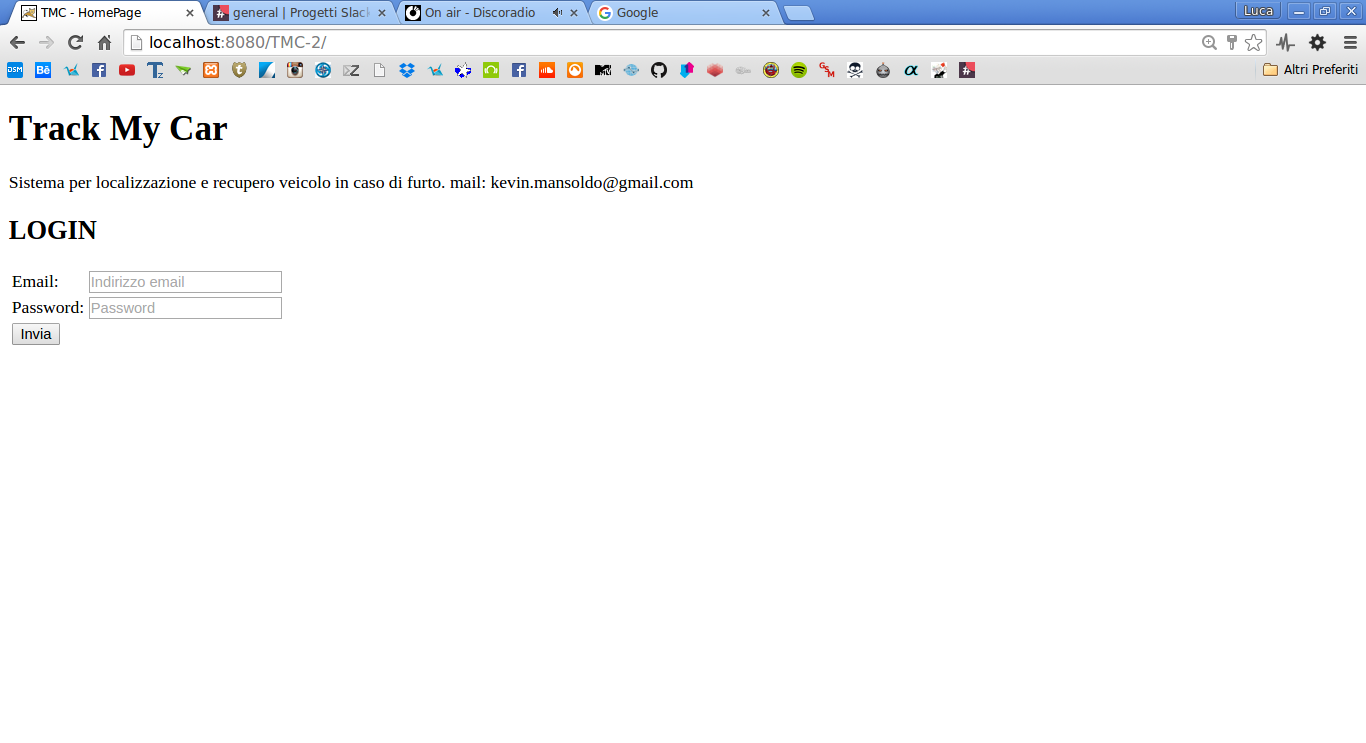
\includegraphics[trim={0 10cm 24.4cm 2.3cm}, clip, scale=1]{login.png}
\caption{Schermata di Login \label{fig:login}}
\end{figure}

\section{Schermata di selezione attività}
L'amministratore e il regular user hanno insiemi di azioni che differiscono tra loro. Infatti, a seconda dei privilegi riservati a ciascun account, sarà possibile accedere ad un numero diverso di funzioni messe a disposizione dall'applicazione. Come da specifiche, per conoscere tutte le operazioni possibili per l'amministratore fare riferimento anche alle funzioni dell'utente regular.

\subsection{Attività Amministratore}
\begin{itemize}
\item \textbf{Gestione utenti} permette di inserire, modificare o eliminare gli utenti a cui è permesso accedere all'applicazione, scegliendo semplicemente l'opzione desiderata.

\item \textbf{Gestione veicoli} permette di inserire, modificare o eliminare i veicoli associati, tramite un menu intuitivo.

\item \textbf{Associazione Utente-Veicolo} dà la possibilità di legare utenti e veicoli, in modo da tracciare poi quello desiderato.

\item \textbf{Impostazione Allarmi} è una funzione che disciplina la velocità massima da superare per ottenere una notifica via mail.

\item \textbf{Gestione utenti} permette di impostare la ricezione di SMS e mail con la posizione del veicolo considerato. L'intervallo di invio è personalizzabile.

\end{itemize}

\begin{figure}[htbp]
\centering
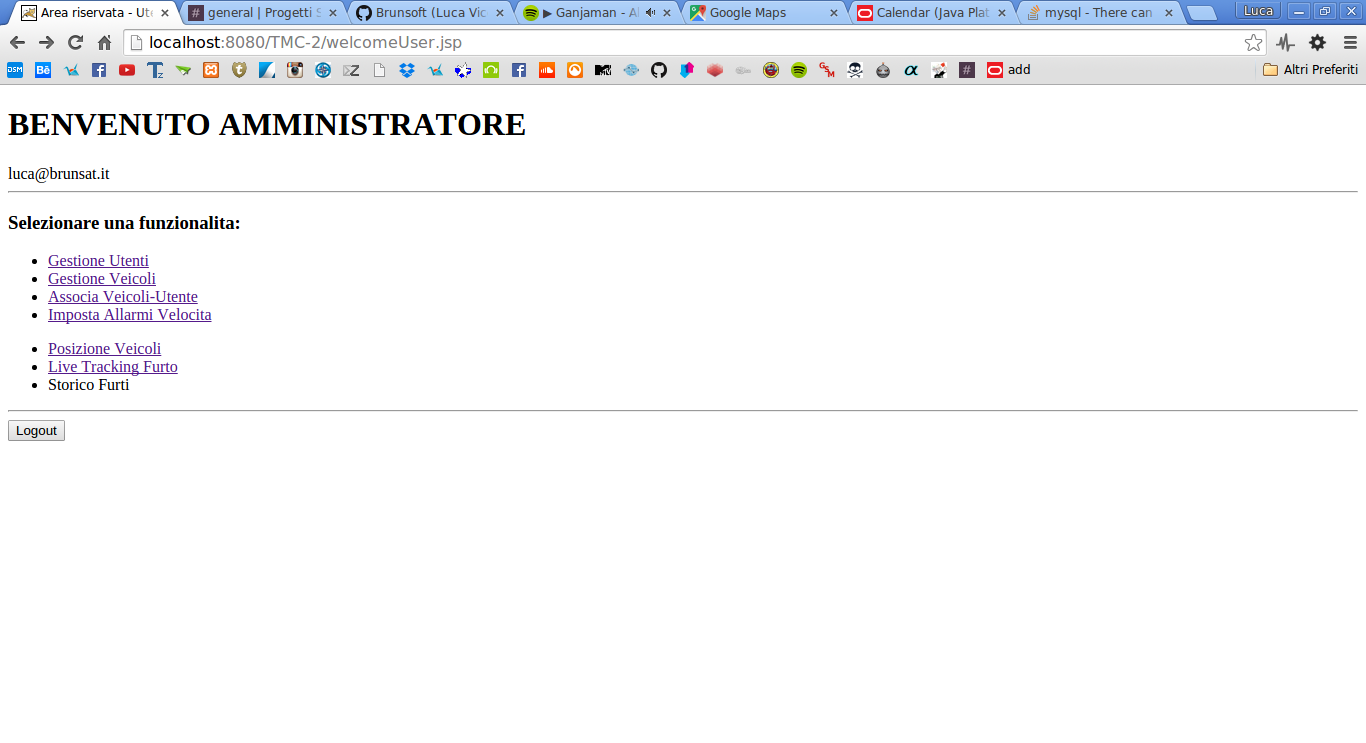
\includegraphics[trim={0 8cm 20.4cm 2.3cm}, clip, scale=0.6]{Home.png}
\caption{Schermata di Login \label{fig:home}}
\end{figure}

\subsection{Attività Regular}
\begin{itemize}
\item \textbf{Visualizza posizione} permette di verificare sulla mappa la posizione attuale del veicolo associato all'utente.

\item \textbf{Live Tracking Furto} permette di seguire in tempo reale lo spostamento del proprio veicolo durante un furto. Fornisce la possibilità di vedere in contemporanea lo streaming in diretta dall'abitacolo.

\item \textbf{Controllo Allarmi Velocità} permette di controllare se sono scattati eventuali allarmi per eccesso di velocità.

\item \textbf{Visualizza Storico Furti} permette di controllare se il veicolo è stato rubato, fornendo i dettagli del furto.

\end{itemize}

\end{document}